%%This is a very basic article template.
%%There is just one section and two subsections.
\documentclass[preprint, nocopyrightspace]{sigplanconf}

% 10-11pt suggested

% \usepackage[dvips, bookmarks, colorlinks=false, pdfborder={0 0 0}, pdftitle={Semester project}, pdfauthor={Ivan Kuraj}, pdfsubject={Improving the finite element assembly procedure using expression template}, pdfkeywords={finite elements, template metaprogramming}]{hyperref} %for creating links in the pdf version and other additional pdf attributes, no effect on the printed document
% \usepackage[final]{pdfpages} %for embedding another pdf, remove if not required

% \usepackage[paper=a4paper,dvips,top=2cm,left=1cm,right=1cm,
%     foot=2cm,bottom=3cm]{geometry}

\usepackage{algorithm}
\usepackage{algorithmic}

\usepackage[pdftex]{graphicx} %for embedding images
\DeclareGraphicsExtensions{.png,.jpg}
\graphicspath{{./img/}}
\usepackage{subfigure}

\usepackage{amsmath}
\usepackage{amsthm}
\newtheorem{definition}{Definiton}

\usepackage{mathpartir}
\usepackage{textcomp}

\newcommand{\cL}{{\cal L}}

\usepackage{xspace}
\newcommand{\LC}{$\lambda$-calculus\xspace}

\newcommand\Lang[1]{\textsl{#1}}

\title{\Lang{InSynth} tool proof translation and (\Lang{Scala}) code generation
\thanks{The work in this paper is focused on an extension of previous version of the InSynth tool developed at EPFL LARA laboratory}}
\subtitle{and integration into the \Lang{Eclipse} IDE}

\authorinfo{Ivan Kuraj\and Tihomer Gvero \and Viktor Kuncak}
{\'{E}cole Polytechnique F\'{e}d\'{e}rale de Lausanne}
{\{first name\}.\{last name\}@epfl.ch}

\begin{document}

\maketitle

\begin{abstract}
Developing modern software applications typically involves composing functionality from existing libraries.
This task is difficult because libraries may expose many methods to the developer.
To help developers in such scenarios, a useful technique can be to synthesize and suggest valid expressions of a given type at a given program point to developer, whenever he asks for it. 

\Lang{InSynth} is a tool for interactive synthesis of code snippets.
 The code synthesis approach behind \Lang{InSynth} is based on the type inhabitation problem with weighted type assignments. 
Weights indicate preferences to certain type bindings; they guide the search and enable the ranking of solutions.

This paper focuses on the ``back-end'' module that has the role of code generation and code snippet output, its interaction with the type inhabitation problem solver module and integration of \Lang{InSynth} into the \Lang{Eclipse} IDE
\footnote{this work contributes to the InSynth tool idea presented in \cite{EPFL-REPORT-170040}}.

The overall experience with \Lang{InSynth} in \Lang{Eclipse} indicates that this approach to synthesizing and suggesting code fragments goes beyond currently available techniques and is a useful functionality of software development environments.
The positive feedback from \Lang{Eclipse} \Lang{Scala} IDE plugin, a popular development environment for \Lang{Scala}, community, promises us that such a feature will bring huge advantage to \Lang{Eclipse} \Lang{Scala} IDE over other IDEs with respect to \Lang{Scala} development.
\end{abstract}
\terms
Languages, Verification
\keywords
Type Inhabitation, Program Synthesis, Typing assist, \Lang{Scala}, \Lang{Eclipse}

\section{Introduction}
\label{sec:introduction}

Libraries are one of the biggest assets for today’s software developers, enabling developers to build on the shoulders of their predecessors. 
Useful libraries often evolve into complex application programming interfaces (\Lang{API}s) with a large number of classes and methods.
It can be difficult for a developer to start using such APIs productively, even for simple tasks \cite{EPFL-REPORT-170040}.
Even if that is not the case, in many popular languages, there exists code constructs of non-negligible size that represent specific combination of API calls and are used very frequently.
Such constructs tend to take developer's precious time to write them and even introduce chances to write them incorrectly.

Existing Integrated Development Environments (\Lang{IDE}s) help developers to use APIs by providing code completion functionality.
For example, an IDE can offer a list of applicable members to a given receiver object, extracted by finding the declared type of the object.
These efforts usually rely on simple syntactical API searches and do not consider the semantics of offered code snippets at the given program point.
Such functionality suggests an interesting general direction of improving modern IDEs:
introduce the ability to search and synthesize type-correct code fragments and offer them as suggestions to the developer (as presented in \cite{EPFL-REPORT-170040}).

In general, existing tools use forward-directed completion in which developer provides a starting value (e.g. a part of an identifier) and the tool bases its search on such starting input.
The \Lang{InSynth} tool uses an observation that developers can productively use backward-directed completion in which, when identifying a computation step, the developer has the type of a desired code construct in mind.
\footnote{Note that this idea can be extended to work without providing the starting type, with languages which provide type inference}
Therefore \Lang{InSynth} does not require the developer to indicate starting fragments of code explicitly. 
Instead, \Lang{InSynth} uses an ambitious approach that considers all values in scope as the candidate leaf values from which expressions can be synthesized.
Forward search typed values are not necessary and may be used to direct the synthesis.

% ******Goals of InSynth******* responsive, modular, \ldots

This paper describes the contributions of the InSynth tool which at the focuses on the Scala language \cite{odersky:scala} and integrates into the Eclipse IDE \cite{eclipse_foundation} as a plugin. 

\subsection{Motivating example}

In the next example we illustrate the functionality of the InSynth tool integrated in Eclipse as a plugin.
Figure \ref{fig:Eclipse_example} depicts a portion of an visible editor in Eclipse IDE and the code suggestions returned by the InSynth tool and how they are shown to the developer. 

\begin{figure}[ht]
\centering
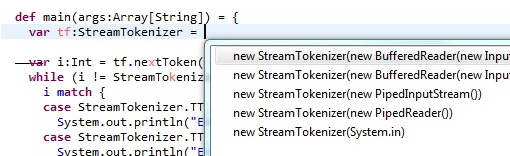
\includegraphics[width=0.45\textwidth]{eclipse}
\caption{InSynth integration in Eclipse}
\label{fig:Eclipse_example}
\end{figure}

The example shows a situation in which the developer has already written some Scala declarations and invokes the Eclipse typing assist functionality which in turn calls the InSynth code synthesis while having the typing pointer at a place for definition of the value which is declared to be of type \textit{StreamTokenizer}.
In such a scenario, InSynth tool is called with the given program context, needed type and visible declarations as the input.
After some specific predefined time working in the background, the developer is provided with a some predefined number of code snippets which were found and ranked the best by InSynth in the given time.
The developer can choose to insert one of such provided code snippets and dramatically reduce the time needed to define the declared \textit{StreamTokenizer} value.
 
% Effectivness in given exmplae, so much terms\ldots blah blah
 
\subsection{Paper outline}

The introduction that sets up the context and a motivating example for the work in this paper for are already given in the Introduction section (Section \ref{sec:introduction}).
We then describe the design of the InSynth tool in terms of modules that InSynth consists of and the phases that are carried out when InSynth tool is invoked by the IDE in Section \ref{sec:design}.
The same section presents design decisions and rationales, algorithms used and implementation aspects involved in InSynth.
In Section \ref{sec:evaluation} a brief evaluation of the InSynth synthesis process and features is given.
Finally the paper is concluded in Section \ref{sec:conclusions} together with mentioning related work to InSynth and also some ideas for the future work.  
 
\section{Design}
\label{sec:design}

In this section we will describe the design of the InSynth tool in high-level of details, introduce the module that uses theorem proving techniques to search for valid code expressions, describe the concepts used in the code generation process and its implementation and justify adopted design decisions along the way. 

\subsection{High-level overview}

InSynth can be thought of as being partitioned into two main modules: 1) proof resolution module and 2) code generation module.
The overview of InSynth design is given in Figure \ref{fig:InSynth_modules}. 

\begin{figure}[ht]
\centering
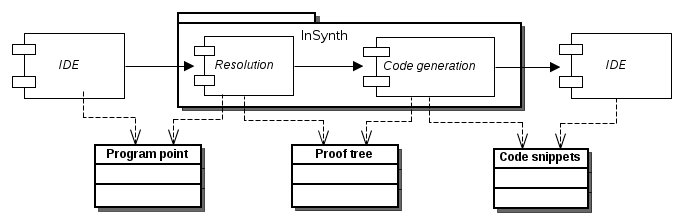
\includegraphics[width=0.45\textwidth]{sav_prez/in_synth_to_export}
\caption{InSynth modules}
\label{fig:InSynth_modules}
\end{figure}

The first, resolution module gets as input program context and a given type to synthesize (which are passed to it from the IDE) and its task is to search for all possible combinations of code constructs so that the resulting expressions are typable in the given program point to the desired type.
This search uses somewhat simplified representation of program context so that it makes utilization of certain theorem proving techniques feasible and efficient.
The output of the proof resolution phase represents proofs that involve simplified language constructs and witness that code expressions of the given type can be constructed.
Such proofs are passed to the code generation module which uses additional information about the program to extrapolate code from them and synthesize code snippets, which when inserted at the desired location in the program evaluate to the given type and the overall program compiles, and feeds them back to the IDE so that they can finally be given as suggestions to the developer.   
\subsection{Resolution}

The resolution phase has the task to search for every possible construction of an expression which has the given type. 
It considers all values in the given scope as the candidate leaf values for expression synthesis.
Considering such a general scenario leads us directly to the type inhabitation problem \cite{EPFL-REPORT-170040,Urzyczyn:1997:ITL:645893.671612}.
\begin{definition}
\label{def:inhabitation_problem}
Type inhabitation problem:
given a desired type $T$, and a type environment $\Gamma$ (a set of values and their types), find an expression $e$ of the type $T$, i.e. find an expression such that $\Gamma \vdash e : T$.
\end{definition}
More specifically, the goal of the resolution phase is to solve the type inhabitation problem - for a input type $T$, to use theorem proving techniques to search for proofs of construction of all valid expressions $e$ of type $T$.
These proofs are then forwarded to the code generations phase which uses them to produce synthesises syntactically correct code snippets.

InSynth gets the necessary inputs from the IDE and the resolution phase computes $\Gamma$ by looking at all program declarations and visible API from the position of the cursor in the editor, looks up $T$ by examining the declared type appearing left of the cursors in the editor and finally solves the type inhabitation problem.

The structure of the phase done by the proof resolution module is depicted in Figure \ref{fig:InSynth_resolution_steps}.

\begin{figure}[ht]
\centering
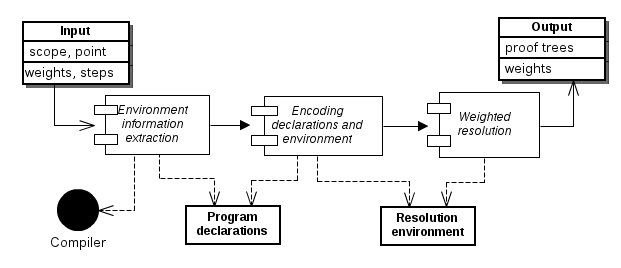
\includegraphics[width=0.45\textwidth]{sav_prez/in_synth_steps}
\caption{InSynth modules}
\label{fig:InSynth_resolution_steps}
\end{figure}

\subsubsection{Environment information extraction}

The first step is the environment information extraction which has the task to extract all usable information about the program.
In the case of Scala programs, the Scala compiler is consulted
\footnote{in the Eclipse IDE integration implementation this is the Scala presentation compiler}
to obtain all local and imported declarations visible at the given program point, which is determined by the typing cursor in the active editor.
The environment extraction automatically assigns weights to all visible declarations according to the distance between the given declaration and the program pointer computed with respect to lines of code and package hierarchy.
The rationale is that the more recent declarations are most likely to be used in the needed expression therefore they should be ranked according to the distance from the given program point.

The number of steps represents a constraint imposed on InSynth in terms of processing time, in order to achieve better responsiveness and ensure a timely termination and suggestions output even in cases of long computations. 

\subsubsection{Encoding the environment}
\label{subsubsec:encoding_the_environment}

The next step of the resolution phase is to encode the environment in the representation which is suitable for the type inhabitation solver to reason about and search for feasible expressions which can be derived from it.

Table \ref{tab:correspondence} shows some examples of how are Scala declarations (and their types) transformed to appropriate representation terms.
The simplified representation of Scala declarations and their types corresponds to the Definition $4.1$ of \textit{ground types} presented in \cite{EPFL-REPORT-170040}.
%PUT HERE def?!
The recursive definition of \textit{ground types} denotes a set of types which include all constants (which correspond to Scala primitive types) and instantiations of constructors (which correspond to Scala generic types) with ground types.
This means that in our resolution process we only consider the instantiated type constructions (e.g. a valid ground type could correspond to Scala types \textit{Int, String, List[String], Map[Int, List[String]]} but not to \textit{Map[X, Y]} where \textit{X, Y} are polymorphic type variables).  

\begin{table}[!ht]
\caption{Correspondence between Scala declarations and proof representation terms}
\centering
{\small
\begin{tabular}{|p{0.22\textwidth}|p{0.20\textwidth}|}
\hline
\textbf{Scala declaration} & \textbf{Proof representation term} \\
\hline
\texttt{val I:Int} & I: $\{\} \rightarrow Int$ \\
\hline
\texttt{def fun(g: Int, f: Int=>Boolean): String} & fun:
$\{ Int, \{ Int \} \rightarrow Boolean \} \rightarrow String$ \\
\hline
\texttt{class A\{ def m(): String \}} & m: $\{A\} \rightarrow String$ \\
\hline
\texttt{class A\{ val s: String \}} & s: $\{A\} \rightarrow String$ \\
\hline
\texttt{def fun(i: Int, c:Char, j: Int): Char} & fun: $(Int, Char) \rightarrow Char$ \\
\hline
% \texttt{def fun(i: Int, c:Char): Char=>Int} & fun: $(Int, Char) \rightarrow Int$ \\
% \hline
\end{tabular}
}
\label{tab:correspondence}
\end{table} 

The environment representation is based on the notion of a type function $f: \{X_1, X_2,\ldots\} \rightarrow Y$ which encodes the information that an expression of type $Y$ can be constructed if a declaration $f$ is used together with expressions of types that belong to the set $X =\{X_1, X_2,\ldots\}$.
More specifically, if expressions $e_i: X_i$ such that $X_i \in X$ where $i=1..|X|$ are available then we can construct an expression $e:Y$ by using those expressions $e_i$ with the declaration $f$ in combination. 

Note that this step produces a representation that sacrifices some information about the language constructs (such as parameter arity, parameter ordering, curring, receiver objects, constructors\ldots) in order to enable more convenient and efficient reasoning with the inhabitation problem solving process (and to make it actually feasible) but also includes corresponding program declarations in order to make the results that use such representation eligible for code reconstruction.

\subsubsection{Weighted resolution}

In order to search for code snippets of the given type, the resolution phase uses theorem proving techniques and reasoning about a similar problem that can be found in type theory, the so-called \textit{type inhabitation problem}, as is defined in Definition \ref{def:inhabitation_problem}.
In the absence of parametric polymorphism, the problem can be seen as the type inhabitation in the simply typed lambda calculus, which is decidable and PSPACE-complete \cite{Urzyczyn:1997:ITL:645893.671612}.

After establishing the connection between program declarations and simplified representation suitable for resolution (or \textit{ground type} terms) in the previous step which encodes the environment (Section \ref{subsubsec:encoding_the_environment}), a calculus for reasoning about the type inhabitation problem is constructed by using only one resolution rule (in  \cite{EPFL-REPORT-170040} it is denoted by \textit{the ground applicative calculus} and it uses multiple rules instead).

\begin{figure}[ht]
\centering{
\inferrule [AppAbs] {\Gamma \vdash f : (\{S_1 \rightarrow T_1\} \cup S_2) \rightarrow T_2 \\ \Gamma \cup \Gamma_{S_1} \vdash h: T_1}
{\Gamma \vdash f(\lambda x_1: ts_1, \ldots \lambda x_n: ts_n. h): S_2 \rightarrow T_2}
\vspace{2mm}
\noindent\begin{minipage}{.26\textwidth}
\begin{equation*}
\Gamma_{S_1} = \{ x_i : ts_i | ts_i \in S_1 \wedge x_i \in \textrm{Fresh} \} 
\end{equation*}
\end{minipage}     
\begin{minipage}{.20\textwidth}  
\begin{equation*}
n = |\Gamma_{S_1}|
\end{equation*}
\end{minipage}
}
\vspace{2mm}
\caption{The calculus rule}
\label{fig:appabs_rule}
\end{figure}

The rule for the calculus construction is depicted in Figure \ref{fig:appabs_rule}.
In combination with the \textit{ground type} representation the \textsc{AppAbs} rule subsumes both the application and abstraction semantics of the lambda calculus (and thus also function composition) in the resolution process.
In order to define starting condition for the resolution process, the \textit{query} \textit{ground type} is added as $q:T \rightarrow \bot$ where $T$ represents the required type of synthesized expressions and $\bot$ represents a fresh type (not usable with the rule for construction of new terms) which is used to denote the end of some expression construction (since $q$, can be instantiated only if an expression of type $T$ itself has been constructed). 

According to the defined calculus the last step of the resolution phase performs the weighted resolution (weights obtained from the information extraction are used to direct the search to more optimal results \cite{EPFL-REPORT-170040}) and produces proof trees which are then used as inputs to the code generation phase. 

\subsection{Code generation}

In this section we will describe the code generation module which has the task of extrapolating and synthesis of code snippets from the proof trees obtained as a result of the resolution phase.

The overview of the code generation phase is given in Figure \ref{fig:InSynth_code_generation}. 

\begin{figure}[ht]
\centering
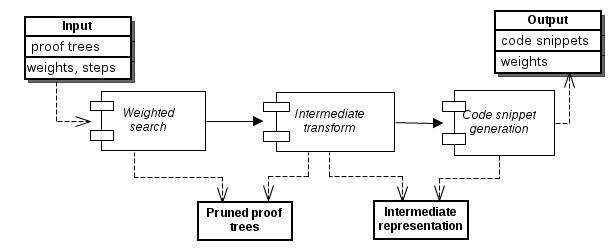
\includegraphics[width=0.45\textwidth]{sav_prez/code_generation_steps}
\caption{InSynth code generation phase}
\label{fig:InSynth_code_generation}
\end{figure}

The code generation phase starts when the resolution phase finished (although its design allows starting the code generation phase as soon as possible and running it in parallel with the resolution phase while receiving partial proof tree updates\footnote{the functionality is considered to be implemented in future work}) and works on the proof tree representation.
The input to the code generation phase besides the constructed proof trees includes the maximal amount of time for the computation (a constraint put on the InSynth tool for responsiveness) and the number of code snippets that should be generated and fed back to the developer.

The first step of the code generation phase is to extract a proof subtree (and transform it into very similar pruned tree representation) which is guaranteed to hold enough information for generation of sufficient number of code snippets with the lowest weight.
The second step takes such pruned proof trees, consults embedded information about the program environment and constructs an intermediate representation tree which holds enough information about the structure of code and program declarations used in the synthesis.
The third step takes the intermediate representation tree and applies transformations which generate a set of Scala code snippets and reports them back to the Eclipse IDE and the developer.

\begin{algorithm}[ht]
\caption{Transformation procedure}
\label{alg:transformation}
\begin{algorithmic}[1]

\REQUIRE{InSynth tree, appropriate $\lambda$ declarations}

\STATE{let $r$ be the root of the InSynth tree} \COMMENT{the root, query node,
has type $(? \rightarrow \bot)$}

\RETURN{Transform($\emptyset$, $r$)}

\end{algorithmic}
\end{algorithm}

The transformation starts with the root node $r$ and an empty typing context
(environment).
The algorithm recursively calls the $Transform$ procedure given in Algorithm
\ref{alg:transform_call}.

% \floatname{algorithm}{Procedure}
% \renewcommand{\algorithmicrequire}{\textbf{Input:}}
% \renewcommand{\algorithmicensure}{\textbf{Output:}}

\begin{algorithm}[ht]
\caption{Transform}
\label{alg:transform_call}
\begin{algorithmic}[1]

\REQUIRE{
	%term $t$, 
	context $\Gamma$, node $n$}
% \COMMENT{The procedure requires:}
% \STATE\COMMENT{since the call is recursive, the term resolved in this
% procedure $x$, will be applied to $t$, i.e. we will have $\lambda$ expression $(t x)$}
\STATE\COMMENT{context $\Gamma$ is the current typing context when resolving the
current term $x$} \STATE\COMMENT{node $n$ is the current node (InSynth SimpleNode) which provides information about resolvent of the current goal type}

\IF{goal is of type $(X \Rightarrow Y)$}
\FORALL{nodes $n'$ with goals of type $Y$}
\FORALL{parameter types $X_i$ in $X$ according to real type}
\STATE{let $x_i$ be fresh variable of type $X_i$}
\ENDFOR
\STATE{let $a$ be an abstraction which takes all parameters in
$X$}
\COMMENT{$a = (\lambda x_1:X_1. (\lambda x_2:X_2. \ldots (\lambda
x_n:X_n.\textrm{ ``\_``})))$}
\FORALL {$t'$ in Transform(\Gamma $\cup (\bigcup_i x_i:X_i)$, $n'$)}
\RETURN {plug $t'$ into the abstraction $a$}
\COMMENT {in place of ``\_``}
\ENDFOR
\ENDFOR
\ENDIF
\IF{goal is of type $X$}
\FORALL{declaration $d$ in declarations in $n$}

\IF{type of $d$ is $X$}
\STATE{return expression of $d$}
\ELSIF{type of $d$ is $X_1 \Rightarrow X_2 \Rightarrow \ldots \Rightarrow X_n
\Rightarrow X$}
\FOR{$i$ in $1..n$}
\IF{there is a leaf child $n'$ of node $n$}
\STATE{let $S_i$ be the set of all variables $v$ such that $v:X_i \in \Gamma$}
\ENDIF
\FORALL{child $n'$ nodes of $n$ with goal type of $X_i$}
% \STATE{find child $n'$ of node $n$ with goal type of $X_1$}
\STATE{let $S_i =$ $S_i$ $\cup$ Transform($\Gamma$, $n'$)}
\ENDFOR
\ENDFOR
\FORALL{combination $x_1, x_2, \ldots, x_n$ of elements $x_1 \in S_1, x_2 \in
S_2, \ldots, x_n \in S_n$}
\RETURN{$x_1$ $x_2$ $\ldots$ $x_n$}
\COMMENT{application of $x_n$ to $x_1$ $\ldots$ $x_{n-1}$}
\ENDFOR
\ENDIF
\ENDFOR
\ENDIF

\end{algorithmic}
\end{algorithm}

\textit{Note:} The line $return$ $x$ in the procedure $Transform$ does not
designate a conventional return call from a function, but rather an indication that such
result $x$ should be returned as one of the results (more
specifically, $Transform$ returns a set of terms which contains all terms which
are prepended with the $return$ command in the Algorithm \ref{alg:transform_call}).

\section{Evaluation}
\label{sec:evaluation}
In this section we will describe important design decisions, properties and functionalities of the code generation phase of InSynth.
Afterwards, we will demonstrate the code generation process with an example of code synthesis for a particular input. 

\subsection{Properties of the code generation}

The most important property of the code synthesis is to generate valid code snippets.
Generated code snippets are valid if under an assumption that proof trees obtained from the resolution phase encode valid expressions (and include correct program declarations), the code generation phase synthesises code snippets that, when inserted at the given program point, typecheck to the given type and the overall program compiles successfully.

\subsubsection{Validity of the code generation phase}

Since the code generation phase consists of three steps, we will enumerate their validity properties individually:
\begin{itemize}
\item weighted search - This step performs pruning of initial proof trees in a way that guarantees at least (needed) $N$ expressions to be combined. The pruned proof tree represents a subset of nodes from the original proof tree in such a way that the structure of that subset is preserved, thus the set of expressions encoded in the pruned proof tree must be a subset of set of expressions encoded in the original proof tree.
\item intermediate transform - The correctness of this step directly depends on the correctness of the \textsc{AppAbs} resolution rule and the correspondence between encoded ground types and program declarations. The intermediate transform directly follows the \textsc{AppAbs} rule by transforming, for each provided declaration its parameters according to the enriched context in the case of parameter type being a function or the original context otherwise. Since the transformation is done according to actual program declarations (types), the intermediate transform trees encodes the correct code structure.
\item code snippet generation - This step relies on properties of the target programming language (Scala) and the transformation is defined by programming language syntactic rules and syntactic sugar instances.
\end{itemize} 

\subsubsection{Completeness}

The second important property of the code synthesis is to be complete, in the sense that the code generation phase should generate all expressions that can be found by the resolution phase (i.e. expressed in the target language) and encoded as ``proofs'' in the input InSynth proof trees.

An interesting treatment of the InSynth code synthesis process is the generation of combinators from the SKI combinatory logic
\footnote{many examples in the literature refer to the combinatory logic as SKI, in spite of the fact that combinators S and K provide completeness of the theory, while I can be expressed as I = S K K}.
Combinatory logic may be viewed as a subset of lambda calculus, the theories are largely the same, becoming equivalent in the presence of the rule of extensionality.
Extensional equality captures the mathematical notion of the equality of functions: two functions are equal if they always produce the same results for the same arguments \cite{Tromp:Lambda}.
The SKI combinatory logic contains the same expressive power as lambda calculus and the logic is variable free, i.e. the abstractions are not part of the logic.
Combinators from the SKI combinatory logic can be composed to produce combinators that are extensionally equal to any lambda term, and therefore, by Church's thesis, to any computable function whatsoever.
The process of obtaining an expression in combinatory logic from any given \LC term can be done with the \textit{abstraction elimination} procedure \cite{Tromp:Lambda}.
In the next section we will see that InSynth is capable of synthesis of combinators from the SKI combinatory logic, when the appropriate input type is given.

In our case the extensional equality of two expressions translates to equivalence of behavior of the two expressions under certain evaluation (reduction \cite{Pierce:2002:TPL:509043}) rules.
Although, due to a specific treatment of declarations (which correspond to application terms as defined in \LC) InSynth synthesis process is not capable of producing every possible code snippet that could be otherwise typed by the developer, it can produce a behaviorally (extensionally) equivalent expression, under the reduction rules of the Scala language.
The specific treatment of declarations limit the expressiveness of the application term to an identifier or a declared term - this means that the expression $(\lambda x:Int. x) $ $5$ (where $5$ represents an appropriate \LC encoding of constant 5) which corresponds to Scala code snippet \textit{((x:Int) =\textgreater} \textit{x)(5)} (which typechecks successfully to \textit{Int}) cannot be produced by InSynth, but its behavioral equivalent $(\lambda x:Int. x)[x \rightarrow 5]$ or in Scala, just the literal \textit{5}, can.

We can conclude that InSynth is indeed capable of producing behaviorally equivalent code to every possible Scala expression, thus every reasonable and useful snippet of code.
\footnote{One interesting remark to notice that under some rather strange (and unpractical) reduction rules (like e.g. full beta-reduction \cite{Pierce:2002:TPL:509043}) $(\lambda x:T. y) z$ may not be behaviorally equivalent to $y[x \rightarrow z]$ in all contexts}

Although the code generation phase should be as expressive as the resolution phase resulting proof trees can be (since the code generation phase consults only proof trees for the code extrapolation and synthesis) the intermediate representation adopted provides the same expression power as \LC (which is Turing-complete \cite{odersky:scala,Pierce:2002:TPL:509043, Tromp:Lambda}) and thus is even more expressible than the proof tree encodings.

\subsection{Demonstration example}

We will give an example of InSynth tool code generation process\footnote{such an example seems the most appropriate since the full integration of the code generation module was not yet possible at the time of writing this paper}, show its intermediate outputs and final results, for the case of the $S$ combinator synthesis, somewhat a combinator from the SKI logic \cite{Tromp:Lambda}.
The $S$ combinator is defined as $(S$ $x$ $y$ $z)$ $=$ $(x$ $z$ $(y$ $z))$ and by its nature it does not require any predefined program declarations, i.e. it can be synthesized with the empty program environment.

The Scala declaration with type of the $S$ combinator (instantiated appropriately with Scala primitive types \textit{Int, Char, String} to be able to be represented as a \textit{ground type}) can be given as

\begin{figure}[ht]
\centering
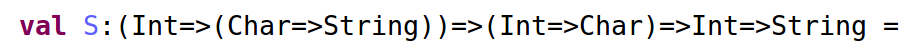
\includegraphics[width=0.45\textwidth]{s_komb}
\end{figure} 

The resulting proof tree as the output of the resolution phase is given in the following figure and it represents nested applications of terms introduced in the context (by the \textsc{AppAbs} rule).

\begin{figure}[ht]
\centering
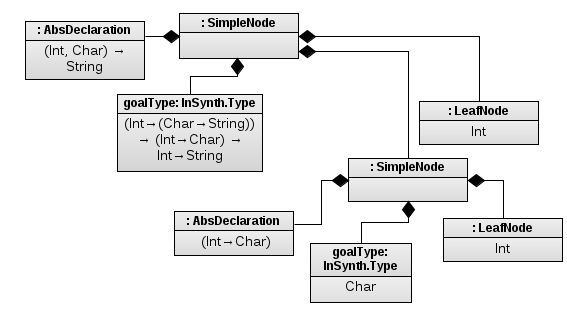
\includegraphics[width=0.40\textwidth]{sav_prez/s_komp_proof_tree}
\end{figure} 

In this particular example the weighted search phase does not affect the tree since there is only one valid expression to be synthesized. 
The intermediate transformation phase produces a tree that in this case completely corresponds to the \LC encoding of the $S$ combinator.

\begin{figure}[ht]
\centering
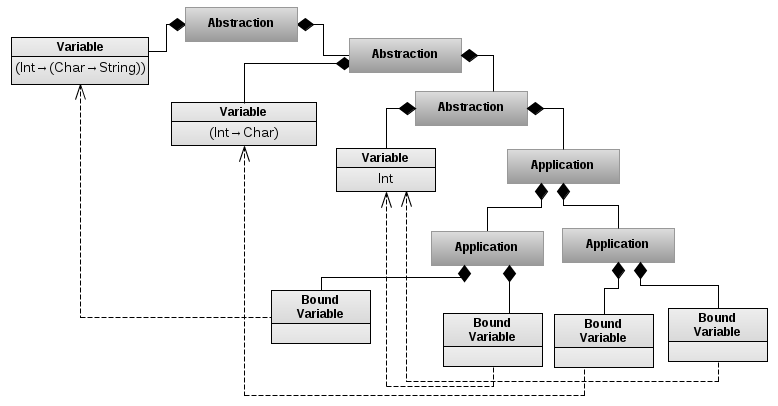
\includegraphics[width=0.45\textwidth]{sav_prez/s_comb_itnermediate}
\end{figure} 

The last step produces of the generation phase produces the scala code which successfully typechecks when inserted as the definition of the declared value \textit{S}. 

\begin{figure}[ht]
\centering
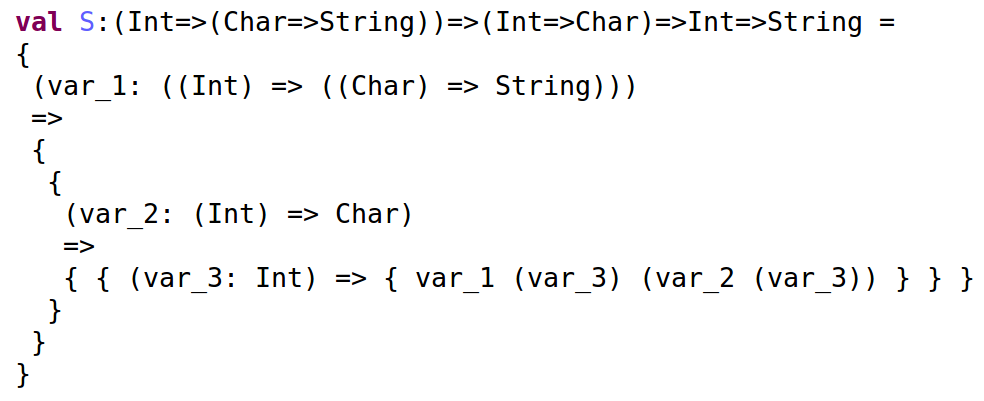
\includegraphics[width=0.45\textwidth]{s_comb_synthesized}
\end{figure} 


\section{Conclusions}
\label{sec:conclusions}
We have described the InSynth tool, mainly its code generation process and its integration with the Eclipse IDE. 
Code generation module is incorporated into the InSynth tool and extends the resolution module which searches for expressions of a given type in a type environment while minimizing a metric on the type binding in order to extrapolate and synthesize the most optimal meaningful code snippets and reports them to the developer.
We implemented the module in three passes and while its implementation offers presented functionality, its design allows convenient extension to support more advanced functionalities.   
Among the key features of the code generation module is the process which takes proof trees from the resolution phase as the input, extracts only necessary information according to specified weight functions and produces code snippets which are valid and appropriately formatted.  

\subsection{Related Work}

There has been work on tools that provide similar functionalities such as InSynth.
There are tools for Haskell that do an API search. The Hoogle \cite{Hoogle} and Hayoo \cite{Hayoo} search engines perform search but rely on user inputs and search only for function names inside APIs. Djinn \cite{Djinn} employs a similar idea as InSynth but does not consider weights for its searches.
Some tools like Prospector \cite{Mandelin:2005:JMH:1065010.1065018} and XSnippet \cite{Sahavechaphan:2006:XMS:1167515.1167508} base their search only on a corpus of collected code rather then searching for possible solutions to be synthesized.

The tool demo on the InSynth tool \cite{demo_paper} suggested the use of theorem prover for classical logic for synthesis. 
In contrast, the current view of our problem is more related to the type inhabitation problem, and intuitionistic logic.
Furthermore, in our approach a method to derive initial weights of declarations is provided, which can prove very important for obtaining useful results.

\subsection{Future Work}

The future work that will happen in a near future would definitely include work on full integration with the Eclipse IDE.
Besides generating expression only when the developer invokes the typing assist after declaring a value with a specified type, InSynth could be used to synthesize code expressions in places such as method call parameters and places where the Scala type inferencer can determine the needed expression type.
Some more advanced features that could be built into the Eclipse IDE would be to include incremental resolution in which user inputs can aid the resolution process and make InSynth much more interactive.

Since InSynth currently supports only type inhabitation problem solving for fully instantiated \textit{ground terms}, one idea would be to extend InSynth to cope with polymorphic types, bounded quantification and reasoning about type variance. 
Very attractive idea is to introduce a corpus of source code (projects written in Scala) and to mine the corpus in order to obtain weighting function for terms and even specific patterns of terms and thus synthesize more useful code snippets.

An implementation of certain semantic checks on the synthesized code would greatly contribute to the practical value of InSynth since by the current process, semantically useless code snippets can be generated (e.g. new \textit{List[Int]().head} can be generated as a code snippet of type \textit{Int}).

% Although InSynth tool still lacks the incorporation and implementation of some useful ideas and features, as such it has proven to be quite useful for practical development, and 

\bibliographystyle{abbrvnat}

\bibliography{main}


\end{document}
